\documentclass{article}
\usepackage{graphicx} % Required for inserting images
\usepackage{setspace}

\usepackage{indentfirst}
\usepackage{amsmath}
\usepackage{amssymb}
\usepackage{varwidth}
\usepackage[margin=1.3in]{geometry}
\usepackage{float}
\usepackage{booktabs}
\usepackage[numbers]{natbib}
\usepackage{breqn}
\renewcommand{\floatpagefraction}{0.8}
\renewcommand{\textfraction}{0.1}
\renewcommand{\topfraction}{0.9}
\renewcommand{\bottomfraction}{0.8}

\title{Optimizing Temporal Regularity of Noise-Induced Spikes in the FitzHugh$-$Nagumo Model}
\author{Kevin Halimman}
\date{March 2026}

\begin{document}

\maketitle

\section{Introduction}
\doublespacing
Neurons communicate through electrical signals known as action potentials, which arise from complex interactions between ionic currents across the cell membrane. The classical model describing this behavior is the Hodgkin$-$Huxley model, which accurately captures the dynamics of ion channels responsible for spike generation. However, the Hodgkin$-$Huxley model consists of four coupled nonlinear differential equations with many parameters to consider, making it extremely difficult to conduct analytical studies utilizing the model.

To better understand the qualitative mechanism underlying neuronal excitability, we use the FitzHugh$-$Nagumo model which still captures the essential dynamics of spike generation while only using two variables: one representing membrane potential and another representing inhibitory processes. And despite the reductions in the model, the FitzHugh$-$Nagumo model still reproduces key behaviors such as threshold dynamics, refractory periods, and oscillatory spiking.

In ideal, deterministic settings, the FitzHugh$-$Nagumo system exhibits dynamics that can be studied using analytical tools from nonlinear dynamical systems theory like phase portraits, nullclines, and limit cycle analysis. For example, the Poincaré$-$Bendixson theorem allows us to determine if there exists a limit cycle (periodic spiking behavior) within some trapping region in a phase space. However, real biological systems are inherently noisy. Ion collisions, thermal fluctuations, and other phenomenon introduce randomness into neuronal dynamics. To account for these effects, we turn to the stochastic FitzHugh$-$Nagumo system, typically formulated as a system of SDEs. 

The goal of this project is to investigate the dynamics of the stochastic FitzHugh$-$Nagumo model using both theoretical analysis and numerical simulations. In particular, we explore how stochastic perturbations affect the regularity of spike trains and modify the long-term dynamics compared to the deterministic case. By combining analytical methods with computational experiments, we illustrate how noise interacts with nonlinear dynamics in excitable biological systems.
\section{Research Question and Hypothesis}
The central research question of this project is: Is there an optimal noise intensity that maximizes the temporal regularity of noise-induced spikes in the excitable FitzHugh$-$Nagumo model? In other words, can action potentials achieve near-periodic behavior in the presence of stochastic perturbations, given that the system is excitable (membrane potential stays at resting potential after initial spike)? Temporal regularity refers to the degree to which successive spikes occur at approximately equal time intervals. If the noise is too weak, spikes may occur very rarely and at irregular times. Conversely, if the noise is too strong, fluctuations may dominate the dynamics and produce highly irregular spiking behavior. Based on this reasoning, we hypothesize that there exists an intermediate noise intensity that produces spikes occurring at approximately equal time intervals, resulting in maximized temporal regularity of noise-induced spiking. This phenomenon is related to the concept of coherence resonance, in which stochastic perturbations can enhance the regularity of oscillations in excitable systems (Pikovsky and Kurths, 1997).

\section{Model Formulation and Simulation}
\subsection{Deterministic FHN}
For the deterministic model, we study the set of equations
\begin{eqnarray}
    \dot{v}&=&v-\frac{v^3}{3}-w+I \\
    \dot{w}&=&\varepsilon(v+a-bw)
\end{eqnarray}
where $v$ represents membrane potential, $w$ represents a recovery/inhibitory process, $I$ represents stimulus current, $a$ represents resting membrane potential, $b$ represents strength of recovery, and $\varepsilon$ represents a time-scale constant. Following convention set by FitzHugh (1961), we set our parameters as $a=0.7$, $b=0.8$, and $\varepsilon=0.08$, putting our system in an excitable regime at small $I$. \cite{fitzhugh1961}

The nullclines of (1) and (2) are
\begin{eqnarray}
    w&=&v-\frac{v^3}{3}+I \\
    w&=&\frac{v+a}{b}
\end{eqnarray}
respectively. Thus, solving for the stationary points would yield different results depending on the input current. For example, when $I=0.1$, there is one stationary point at approximately $(-1.14, -0.55)$. When $I=0.5$, there is one stationary point at approximately $(-0.80, -0.13)$. When $I=0.9$, one stationary point at approximately $(0.10, 1.0)$. These values of $I$ are chosen to fall within a biological range of $I\in [0,1.5]$ following the parameter study conducted by Hanan et al (2020). \cite{hanan2020} The stability of these points can be determined by analyzing the Jacobian matrix of the system at each point. Consider the Jacobian matrix:
\begin{equation}
    J=\begin{bmatrix}1-v^2 & -1 \\
\varepsilon & -\varepsilon b\end{bmatrix}
\end{equation}
We compute the eigenvalues of $J$ at each stationary point to determine their stability. For $I=0.1$, the eigenvalues are 
complex conjugates with negative real parts, indicating that the stationary point is a stable focus. In this regime, the 
system is excitable such that trajectories remain near the equilibrium under small perturbations, but sufficiently large 
perturbations can trigger a spike (action potential) before returning to rest. For $I=0.5$, the eigenvalues are complex 
conjugates with positive real parts, indicating that the stationary point is an unstable focus. Similarly, for $I=0.9$, 
the eigenvalues are real and positive, corresponding to an unstable node. In the cases $I=0.5,0.9$, the equilibrium has 
lost stability through a Hopf bifurcation at some $I=I_H$. We know this because at $I=0.1$, the eigenvalues are complex 
conjugates with negative real parts and at $I=0.5$, they are complex conjugates with positive real parts. By the 
Intermediate Value Theorem, there must be some critical value of $I$ between $0.1$ and $0.5$ where the real part of the 
eigenvalues crosses zero, indicating a Hopf bifurcation. But we still don't know what the long-term behavior of the system is for $I>I_H$. Does the membrane potential diverge to 
infinity? From a biological standpoint, probably not. Does it approach a limit cycle? This is more likely but it motivates a more rigorous analysis.

We can use the Poincaré$-$Bendixson theorem to help us analyze long-term behavior here. 
The theorem states that if a trajectory of a 2D dynamical system is confined to a compact region $K$ and does not contain 
a stationary point, the $\omega$-limit set of that trajectory must be a limit cycle. Given that for $I > I_H$, the unique 
stationary point $(v^*, w^*)$ is an unstable focus or node, we can satisfy the theorem's conditions by constructing a 
compact annular trapping region $\mathcal{A}$ that excludes a small neighborhood $U_\epsilon(v^*, w^*)$. 

To explicitly define this trapping region, we introduce an energy function for the FitzHugh$-$Nagumo system. 
Let $(v^*, w^*)$ denote the unique stationary point satisfying 
\begin{equation}
v^* - \frac{(v^*)^3}{3} - w^* + I = 0, \quad w^* = \frac{v^* + a}{b}.
\end{equation}
Define the total energy function as the weighted quadratic distance from the stationary point:
\begin{equation}
E(v, w) = \frac{1}{2}(v - v^*)^2 + \frac{1}{2\varepsilon}(w - w^*)^2.
\end{equation}
Taking the time derivative along trajectories of the system gives
\begin{align}
\frac{dE}{dt} &= (v - v^*)\dot{v} + \frac{1}{\varepsilon}(w - w^*)\dot{w} \\
             &= (v - v^*)\left(v - \frac{v^3}{3} - w + I\right) + \frac{1}{\varepsilon}(w - w^*)\varepsilon(v + a - bw) \\
             &= (v - v^*)\left(v - \frac{v^3}{3} - w + I\right) + (w - w^*)(v + a - bw).
\end{align}
Using $w^* = \frac{v^* + a}{b}$ from (6), we rewrite $v + a - bw = v - v^* - b(w - w^*)$. Then
\begin{align}
\frac{dE}{dt} &= (v - v^*)\left(v - \frac{v^3}{3} - w + I\right) + (w - w^*)\left(v - v^* - b(w - w^*)\right) \\
             &= (v - v^*)\left(v - \frac{v^3}{3} - w + I + w - w^*\right) - b(w - w^*)^2 \\
             &= (v - v^*)\left(v - \frac{v^3}{3} + I - w^*\right) - b(w - w^*)^2.
\end{align}
Since $v^* - \frac{(v^*)^3}{3} + I - w^* = 0$ at equilibrium, we have $I - w^* = \frac{(v^*)^3}{3} - v^*$, so
\begin{equation}
\frac{dE}{dt} = (v - v^*)\left(v - \frac{v^3}{3} - v^* + \frac{(v^*)^3}{3}\right) - b(w - w^*)^2.
\end{equation}
Although $-b(w - w^*)^2 < 0$, we still cannot guarantee that $\frac{dE}{dt} < 0$. But to leading 
order, $v-\frac{v^3}{3}$ behaves like $-\frac{v^3}{3}<0$ for large $|v|$, so the first term also becomes negative for 
sufficiently large $|v|$. Therefore, there exists some radius $R$ such that $\frac{dE}{dt} < 0$ on the boundary 
$E(v, w) = R$, given that $R$ is large enough to accomodate a sufficiently large $|v|$.

Thus, the compact region
\begin{equation}
    K = \{(v, w) : E(v, w) \leq R\}
\end{equation}
for sufficiently large $R$ forms a trapping region: trajectories that start inside $K$ remain in $K$ for all future time and trajectories that start outside $K$ eventually enter $K$ because if a trajectory starts at radius $r>R$, $|v|$ will still be large enough to ensure $\frac{dE}{dt} < 0$. And then because the unique stationary point $(v^*, w^*)$ in this regime is an unstable focus, we can exclude a small neighborhood around it, and the Poincaré$-$Bendixson theorem guarantees the existence of a limit cycle in the annular region 
\begin{equation}
    \mathcal{A} = K \setminus U_\epsilon(v^*, w^*).
\end{equation}
with inner radius $\epsilon$ and outer radius $R$. 
This limit cycle corresponds to the periodic spiking behavior observed in the neuron for $I > I_H$.

To test this claim, we can run various simulations and study the plots generated. Firstly, we can plot the phase portraits of the system for each value of $I$. The phase portraits show the trajectories of the system in the $v$-$w$ plane, along with the nullclines and stationary points. 
\begin{figure} [H]
    \centering
    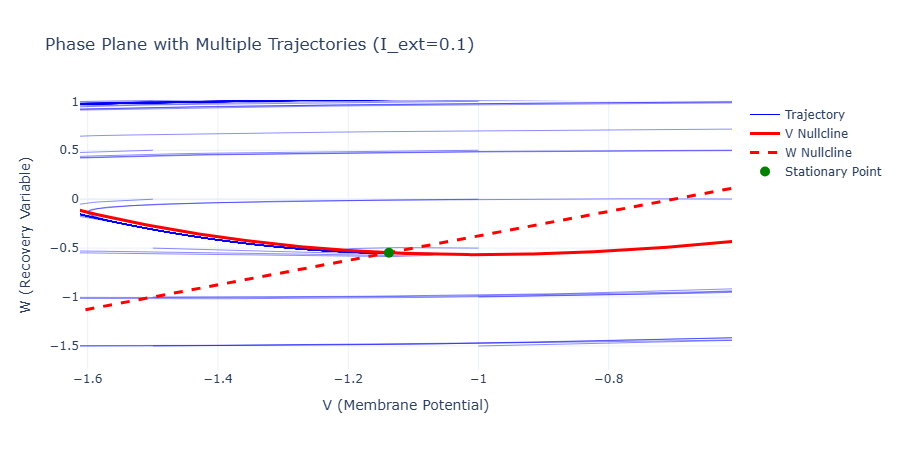
\includegraphics[width=0.8\textwidth]{phase_plane_0.1_zoom.png}
    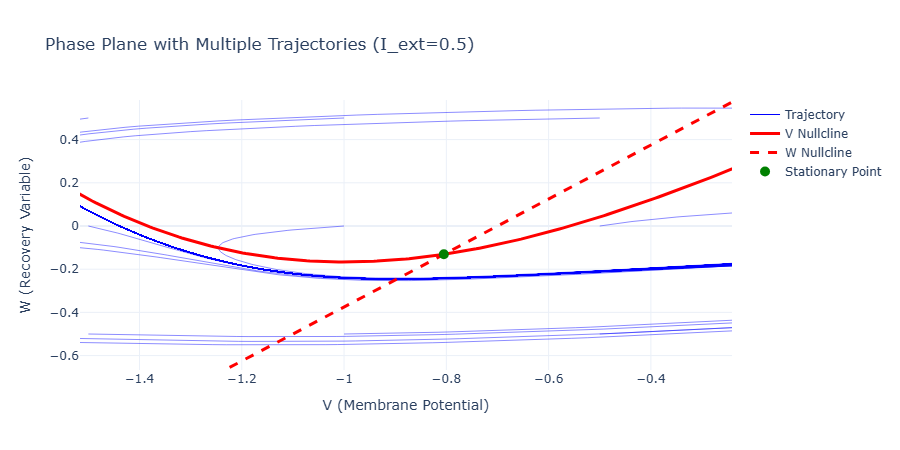
\includegraphics[width=0.8\textwidth]{phase_plane_0.5_zoom.png}
    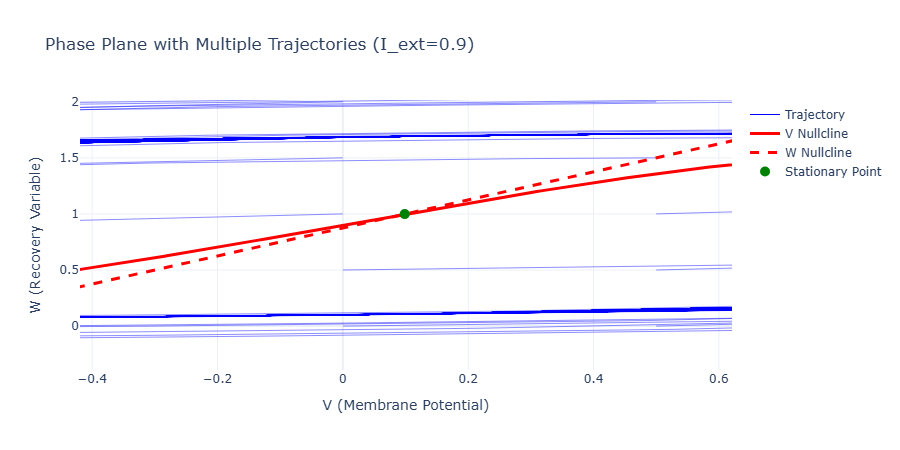
\includegraphics[width=0.8\textwidth]{phase_plane_0.9_zoom.png}
    \caption{Zoomed phase portraits of the deterministic FitzHugh$-$Nagumo model for different values of input current $I$. The nullclines are shown in red lines and the stationary points are marked with dots. The trajectories illustrate the dynamics of the system in the $v$-$w$ plane.}
\end{figure}
For $I=0.1$, we observe that trajectories spiral towards the stable  focus, indicating that the system is in an 
excitable regime. For $I=0.5$, we observe that trajectories spiral around the unstable focus. And similarly,
for $I=0.9$ we see that trajectories also never settle at the stationary point. These phase portraits 
provide insight into the qualitative dynamics of the system under different input currents and essentially confirm our
previous analysis of the stability of the stationary point.

To gain a further understanding of how the system evolves over time, we can also plot the time series of $v$ and $w$ 
for each value of $I$. The time series show how the membrane potential and recovery variable change over time, 
providing insight into the temporal dynamics of the system. We see that from $I=0$ to $I=0.3$, the system 
stays at resting membrane potential after the initial spike. However, for $I>0.3$, the system exhibits unstable to 
periodic spiking behavior which confirms our claims about the system's oscillatory behavior at $I>I_H$.
\begin{figure} [H]
    \centering
    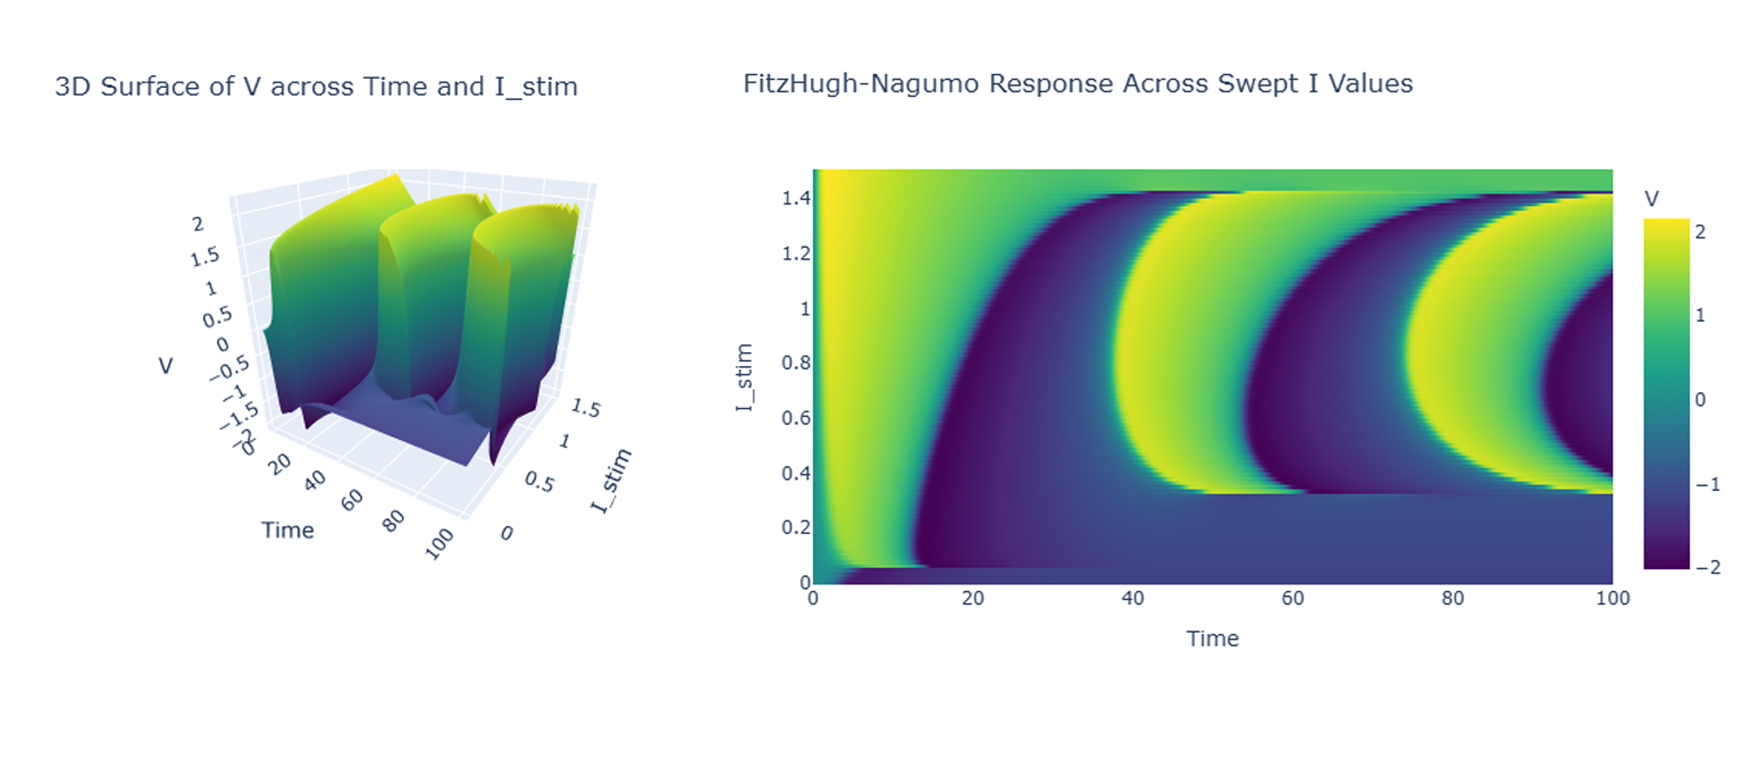
\includegraphics[width=1\textwidth]{CompositeFigure4-5.png}
    \caption{Time series of the membrane potential $v$ for different values of input current $I$. The plots illustrate how the system evolves over time, showing the transition from resting state to periodic spiking behavior as $I$ increases from 0 to 1.5.} 
\end{figure}
\begin{figure} [H]
    \centering
    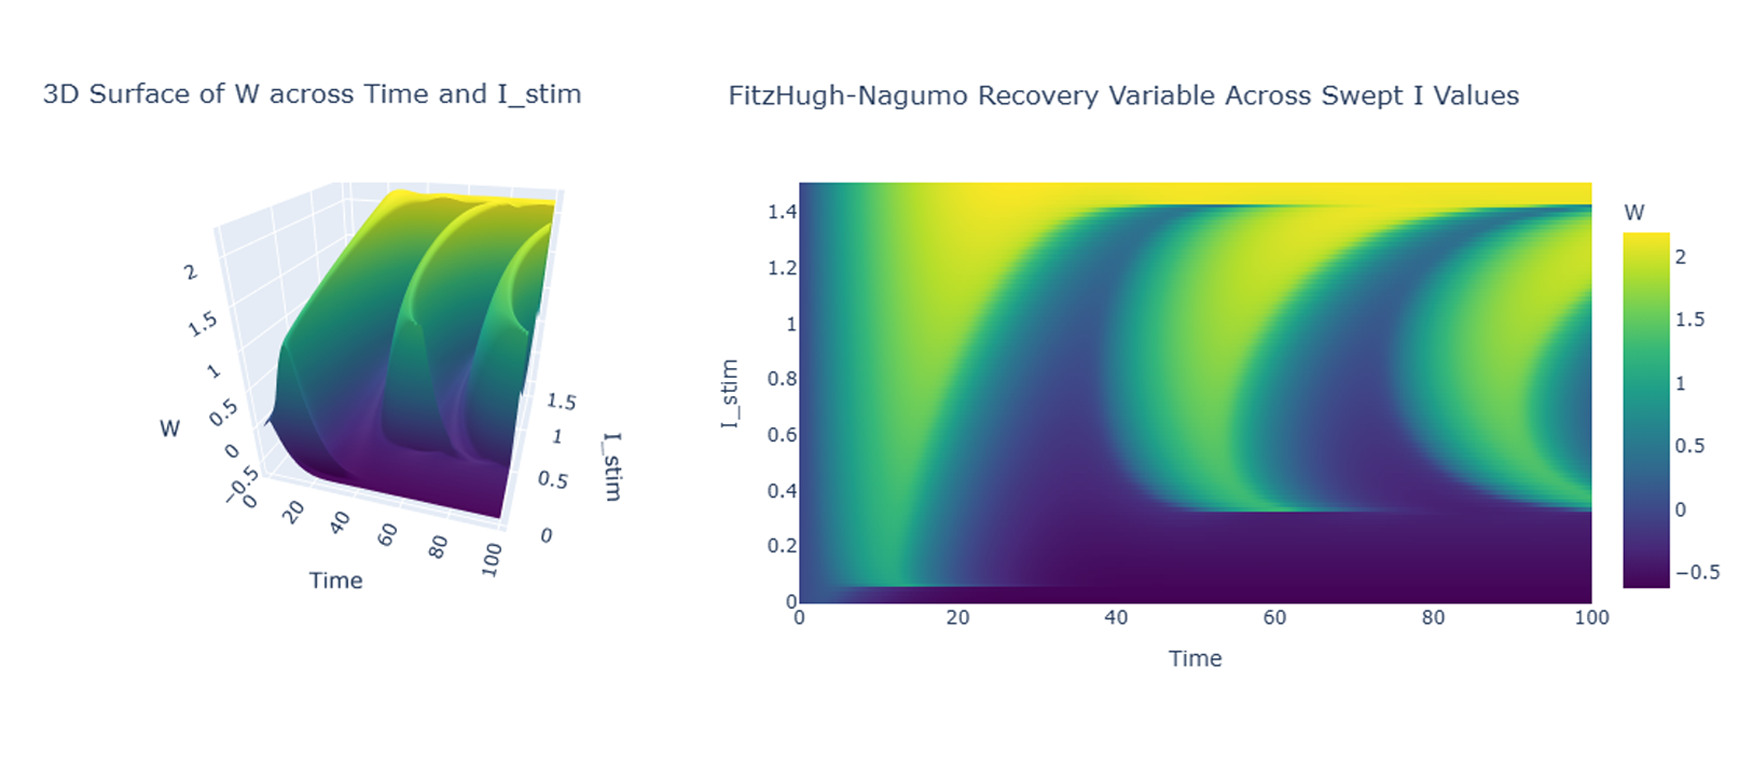
\includegraphics[width=1\linewidth]{CompositeFigure6-7.png}
    \caption{Time series of the recovery variable $w$ for different values of input current $I$.}
    \label{fig:placeholder}
\end{figure}

The deterministic system therefore exhibits two qualitatively unique regimes of behavior depending on the value of $I$: an excitable regime for low input currents and an oscillatory regime for medium to high input currents. The excitable regime is particularly important for our study because it is in this regime that noise can induce spikes. In real neurons, such perturbations often arise from random fluctuations caused by ion channel noise or other stochastic processes, thus motivating our extension of the deterministic formulation to a stochastic version of the model.
\subsection{Stochastic FHN}
For the stochastic model, we study the set of equations
\begin{eqnarray}
    dv&=&\left(v-\frac{v^3}{3}-w+I\right)dt+\sigma dW_t \\
    dw&=&\varepsilon(v+a-bw)dt
\end{eqnarray}
where $\sigma$ represents the volatility or noise intensity and $W_t$ represents a standard Wiener process. Notice that when we take $\sigma =0$, our system mirrors the deterministic case. The noise term $\sigma dW_t$ introduces stochastic perturbations to the membrane potential, which can lead to noise-induced spiking behavior even when the system is in a resting state in the deterministic case. 

To investigate the effect of noise on the dynamics of the system, we can perform numerical simulations of the stochastic FitzHugh$-$Nagumo model for different values of $\sigma$. Most commonly, the Euler-Maruyama method is used to approximate the solution of the SDEs, which involves discretizing time into small steps and iteratively updating the values of $v$ and $w$. Thus, we will use
\begin{equation}
    v_{n+1}=v_n+\left(v_n-\frac{v_n^3}{3}-w_n+I\right)\Delta t+\sigma \sqrt{\Delta t} Z_n
\end{equation}
where we have approximated the increment $\Delta W_n$ as $\sqrt{\Delta t} Z_n$ based on the properties of Brownian motion and used $Z_n$ as standard normal random variable $N(0,1)$. We can also update $w$ using the deterministically since it does not have a noise term:
\begin{equation}
    w_{n+1}=w_n+\varepsilon(v_n+a-bw_n)\Delta t
\end{equation}
Literature suggests that $\sigma=0.2$ is considered strong noise so we will sweep $\sigma$ from $0.0$ to $0.4$ to stay within a physiologically relevant range. Additionally, we set $I=0.1$ so that the deterministic system remains at a stable resting equilibrium (excitable regime), allowing us to isolate noise-induced spikes and test whether an intermediate noise intensity maximizes their temporal regularity (coherence resonance). 

For each value of $\sigma$, we will run 60 trials of the simulation to compute statistics on the inter-spike intervals (ISIs) and spike counts, which will allow us to analyze the temporal regularity of the noise-induced spikes. Then we can plot the mean coefficient of variation (CV) of the ISIs and the mean spike count as a function of $\sigma$ to investigate whether there is an optimal noise intensity that maximizes temporal regularity. Note that we define the CV of ISIs as
\begin{equation}
    CV = \frac{\sigma_{ISI}}{\mu_{ISI}}
\end{equation}
where $\sigma_{ISI}$ is the standard deviation of the ISIs and $\mu_{ISI}$ is the mean of the ISIs. A lower CV indicates more regular spiking behavior, while a higher CV indicates more irregular spiking behavior. Therefore, if there exists an optimal noise intensity that maximizes temporal regularity, we would expect to see a minimum in the mean CV as a function of $\sigma$, the noise intensity.

We now examine the results of the stochastic simulations across the range of noise intensities. For each value of $\sigma$, the model was simulated for multiple trials and the resulting spike statistics were aggregated to compute the mean coefficient of variation (CV) of the inter-spike intervals and the mean spike count.

Figure 4 shows the mean CV of the inter-spike intervals as a function of the noise intensity. For very small values of $\sigma$, the system rarely produces spikes because the deterministic system lies in a resting state. As a result, the few spikes that do occur are highly irregular, leading to large variability in the CV. As the noise intensity increases, the system begins to spike more regularly due to noise-induced threshold crossings.

Initially, the CV shoots up as $\sigma$ increases, which is to be expected since the system transitions from a non-spiking state to a spiking state. However, as $\sigma$ continues to increase, the CV starts to decrease, indicating that the spikes are becoming more regular. This phenomenon is somewhat related to coherence resonance but we ultimately don't observe a clear minimum in the mean CV as a function of $\sigma$. Instead, the CV appears to plateau at intermediate to high noise intensities, suggesting that while noise can enhance the regularity of spiking to some extent, there may not be a well-defined optimal noise intensity that maximizes temporal regularity in this particular system.


\begin{figure}[H]
\centering
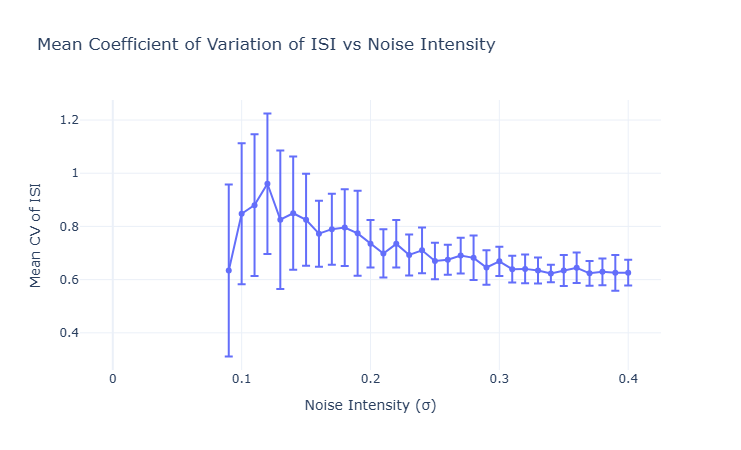
\includegraphics[width=0.75\linewidth]{cv_vs_sigma.png}
\caption{Mean coefficient of variation (CV) of the inter-spike intervals as a function of noise intensity $\sigma$. Error bars represent the standard deviation across trials.}
\label{fig:cv_vs_sigma}
\end{figure}
It turns out that the absence of a clear coherence resonance minimum can be attributed to the specific parameter regime used in our study. The foundational work by Pikovsky and Kurths on coherence resonance in excitable systems demonstrated that the phenomenon is most observable when the system is close to the Hopf bifurcation threshold \cite{pikovsky1997coherence}. In our case, the input current $I = 0.1$ places the deterministic system deeply in the excitable regime, but at some distance from the critical value $I_H \approx 0.33$ where the equilibrium loses stability. Thus, our parameter regime differs significantly from that used in many studies observing pronounced CV minimization. For example, Pikovsky and Kurths used a smaller time-scale parameter $\varepsilon = 0.01$ compared to our value of $\varepsilon = 0.08$, which creates a larger separation between charging and recovery timescales \cite{pikovsky1997coherence}. Similarly, Casado (2002) showed analytically that the optimal noise intensity required to observe coherence resonance decreases as the distance between the bifurcation parameter and its critical value decreases \cite{casado2002resonance}. Additionally, the noise intensity needed to induce spikes at our working point is relatively high because the system is far from threshold, which causes the CV to plateau rather than achieve a distinct minimum \cite{longtin1997intrinsic}. These findings suggest that clearer coherence resonance behavior might be observable by operating closer to the Hopf bifurcation (e.g., $I \approx 0.25$) or using a smaller time-scale separation parameter. 

To further understand the effect of noise on the activity of the system, we also examine the mean spike count as a function of noise intensity. The results are shown in Figure 5. As expected, the number of spikes increases roughly monotonically with increasing $\sigma$. When $\sigma$ is small, the noise is insufficient to push the membrane potential past the excitation threshold, resulting in few or no spikes. As the noise intensity increases, stochastic fluctuations increasingly drive the system across the threshold, leading to more frequent spiking events.

\begin{figure}[H]
\centering
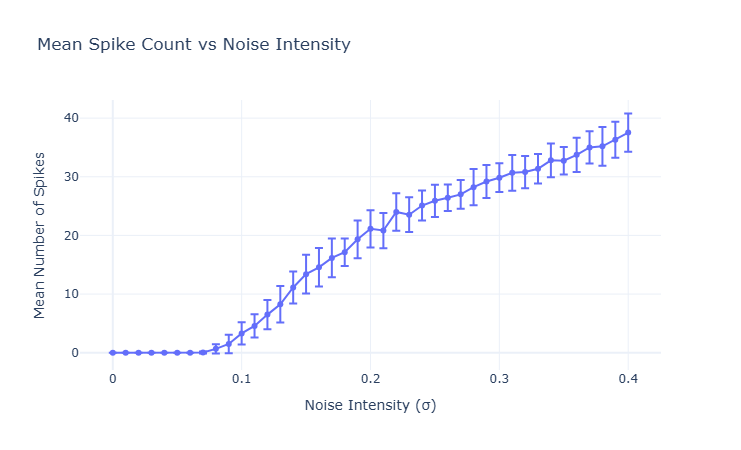
\includegraphics[width=0.65\linewidth]{spikecount_vs_sigma.png}
\caption{Mean spike count as a function of noise intensity $\sigma$. Error bars represent the standard deviation across trials.}
\label{fig:spikecount_vs_sigma}
\end{figure}

Finally, to illustrate how the qualitative behavior of the membrane potential changes with noise intensity, sample trajectories of the membrane potential $v(t)$ are shown for several representative values of $\sigma$ in Figure 6. At very low noise levels, the system remains near its resting state with only small fluctuations. As $\sigma$ increases, occasional excursions away from the resting state occur, producing isolated spikes. For larger values of $\sigma$, the system exhibits sustained stochastic spiking with increasingly frequent firing events.

These trajectories highlight how noise can fundamentally alter the dynamical behavior of an excitable system. Even though the deterministic model remains at rest, stochastic perturbations can induce repeated threshold crossings and generate spike trains.

\begin{figure}[H]
\centering
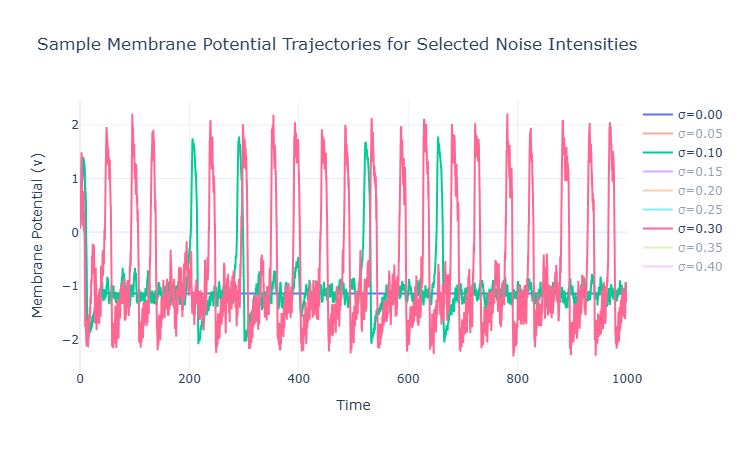
\includegraphics[width=0.9\linewidth]{sample_trajectory.png}
\caption{Sample membrane potential trajectories $v(t)$ for selected values of the noise intensity $\sigma$. Increasing noise leads to more frequent noise-induced spikes.}
\label{fig:trajectories}
\end{figure}

\section{Conclusion}

In this paper, we investigated the dynamics of both deterministic and stochastic FitzHugh$-$Nagumo models to understand how noise affects spike regularity in excitable neurons. Our key findings are summarized as follows.

First, using the Poincaré$-$Bendixson theorem with an energy function approach, we proved the existence of a limit cycle in the deterministic system for input currents above the Hopf bifurcation threshold $I > I_H$. This confirms that the deterministic model exhibits periodic spiking behavior in the oscillatory regime.
Second, our numerical simulations reveal that noise can induce sporadic spiking even when the deterministic system resides in a stable resting state (at $I = 0.1$). At low noise intensities, spikes are rare and highly irregular. As noise increases, so does spike frequency, and the CV decreases as spike timing becomes more regular.
Third, unlike classical coherence resonance studies, we did not observe a well-defined minimum in the CV versus noise curve. Rather, the CV plateaus at intermediate to high noise levels. We attribute this to our choice of parameters: working at $I = 0.1$ places the system far from the Hopf bifurcation, and using $\varepsilon = 0.08$ provides weaker time-scale separation than the $\varepsilon = 0.01$ typically used in coherence resonance studies \cite{pikovsky1997coherence}. This suggests that to observe pronounced coherence resonance in the FHN model, one should operate closer to the excitability threshold and utilize a smaller time-scale separation parameter.
From a biological standpoint, our findings highlight how noise can play a constructive role in neuronal dynamics by inducing regular spiking patterns in otherwise quiescent systems. This has implications for understanding how neurons communicate and process information.

But more broadly, these findings have direct implications for neuromorphic computing systems that utilize spiking neural networks, a type of artificial neural network that mimics the behavior of biological neurons. Our results suggest several design principles.
At our operating point ($I = 0.1$, deep in the excitable regime), noise can induce occasional spiking even in the absence of constant input currents. This enables event-driven architectures where spikes occur only when noise crosses threshold, potentially reducing power consumption compared to continuously-clocked systems. This allows for efficient information processing in low-power neuromorphic chips, where stochasticity can be harnessed to generate sparse, event-driven activity patterns. A great example of technology that would benefit from this approach are seismic monitors that only spike in response to significant events rather than continuously monitoring signals \cite{indiveri2011neuromorphic}.
Moreover, our finding that the CV plateaus rather than exhibiting a sharp minimum indicates the system is robust to parameter variations. This is practically advantageous for hardware, where noise levels may fluctuate with temperature or manufacturing variations. Thus, our study directly informs design choices to mimic our model parameters.

Overall, our investigation of the FitzHugh$-$Nagumo model demonstrates how noise can induce and modulate spiking behavior in excitable systems. By combining theoretical analysis with numerical simulations, we provide insights into the interplay between stochastic perturbations and nonlinear dynamics in neuronal models. Future work could explore other parameter regimes, different types of noise, or implementations informed by our findings in neuromorphic hardware to further understand and harness noise-induced phenomena in excitable systems.
\bibliographystyle{plainnat}
\bibliography{references}

\end{document}